\documentclass{article}
\usepackage{booktabs}
\usepackage[a4paper, top=2cm, bottom=2cm, left=2.6cm, right=2.6cm]{geometry} % Keep only one geometry package
\usepackage[utf8]{inputenc}
\usepackage{amsmath}
\usepackage{eurosym}
\usepackage[T1]{fontenc}
\usepackage[french]{babel}
\usepackage{graphicx}
\usepackage{caption}
\usepackage{float}
\usepackage{multirow}
\usepackage{blindtext}
\usepackage{hyperref}
\usepackage{setspace} % Required for \onehalfspacing
\usepackage{subcaption}


\begin{document}

\normalsize

\begin{titlepage}
\begin{center}

\includegraphics[width=0.7\textwidth]{images_titre/ensai_logo.png}\\[2.0 cm] 

\rule{\linewidth}{0.4mm} \\[0.4cm]
{\Large\bfseries Quelles circonstances sont associées à l’expression de signes cliniques respiratoires des porcs en croissance en élevages alternatifs?}\\[0.2cm]
\rule{\linewidth}{0.4mm}\\[3cm]

\begin{flushleft} \large
\emph{\underline{Étudiants:}}\\[0.2cm]
Antoni \textsc{Guàrdia Sanz} \\
Clément \textsc{Yvernault-Collet} \\
Marius \textsc{Vinclair}\\
Xavier \textsc{Braquaval}\\
\end{flushleft}

\begin{flushright} \large
\emph{\underline{Tutrice:}} \\[0.2cm]
Christelle \textsc{Fablet} \\[0.6cm]
\end{flushright}

\vfill
{\large \today}
\end{center}
\end{titlepage}

\newpage
\tableofcontents 
\newpage

\section{Introduction}
\subsection{Introduction du sujet}
\subsection{Description de la base de données}
\newpage
\section{Etude des variables respiratoires}
Dans cette section, on se propose d’analyser les relations entre les variables caractérisant la respiration des porcs, en particulier les fréquences d’éternuements et de toux en engraissement et post-sevrage, afin d’identifier les liens existants. L’objectif est de regrouper ces variables et de simplifier l’étude en réduisant leur complexité.

\subsection{Présentation et caractérisation des variables respiratoires}
Dans cette partie, nous présentons et caractérisons les variables respiratoires mesurées chez les porcs. L'objectif est de mieux comprendre la répartition de ces données et d'identifier d'éventuelles particularités dans le comportement respiratoire des porcs.
%\begin{table}[h]
%    \centering
%    \begin{tabular}{lcccc}
%        \toprule
%        & Eter. PS & Eter. Eng & Toux PS & Toux ENG \\
%        \midrule
%        Min.   & 0.0000  & 0.0000  & 0.0000   & 0.000  \\
%        Q1 & 0.5401  & 0.0000  & 0.0000   & 0.000  \\
%        Medianne  & 3.1429  & 0.7587  & 0.7767   & 1.524  \\
%        Moyenne    & 9.0345  & 2.1773  & 6.2761   & 7.119  \\
%        Q3 & 10.0000 & 2.9241  & 5.5303   & 8.472  \\
%        Max.    & 88.8889 & 16.1290 & 137.0370 & 70.000 \\
%        NA's    & 1       & 4       & 1        & 4      \\
%        \bottomrule
%    \end{tabular}
%    \caption{Caractérisation des variables respiratoires}\label{tab:summary_stats}
%\end{table}

\begin{figure}[H]
    \centering
    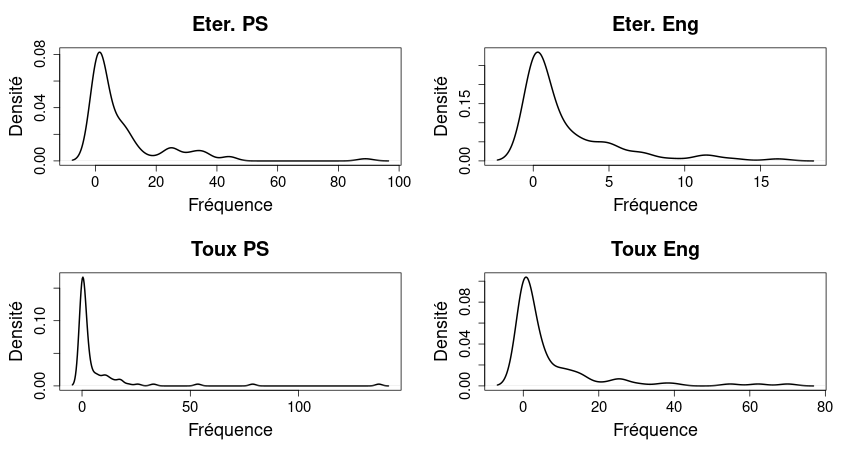
\includegraphics[width=\textwidth]{img_var_resp/dens_var_resp.png}
    \caption{Densité des variables respiratoires (BP\protect\footnotemark\ \text{: }nrd0\protect\footnotemark)}\label{fig:dens_resp}
\end{figure}

\addtocounter{footnote}{-1}
\footnotetext[\thefootnote]{Bande passante.} 
\addtocounter{footnote}{1}
\footnotetext[\thefootnote]{La méthode \texttt{nrd0} fait référence à la largeur de bande de référence normale.}

Notons que dans (\ref{fig:dens_resp}) les quatre variables respiratoires présentent une forte concentration de la densité autour de 0, ce qui reflète un bon état respiratoire global chez les porcs étudiés. Cependant, certains élevages montrent des exceptions où cette tendance générale n'est pas observée.

\begin{figure}[H]
    \centering
    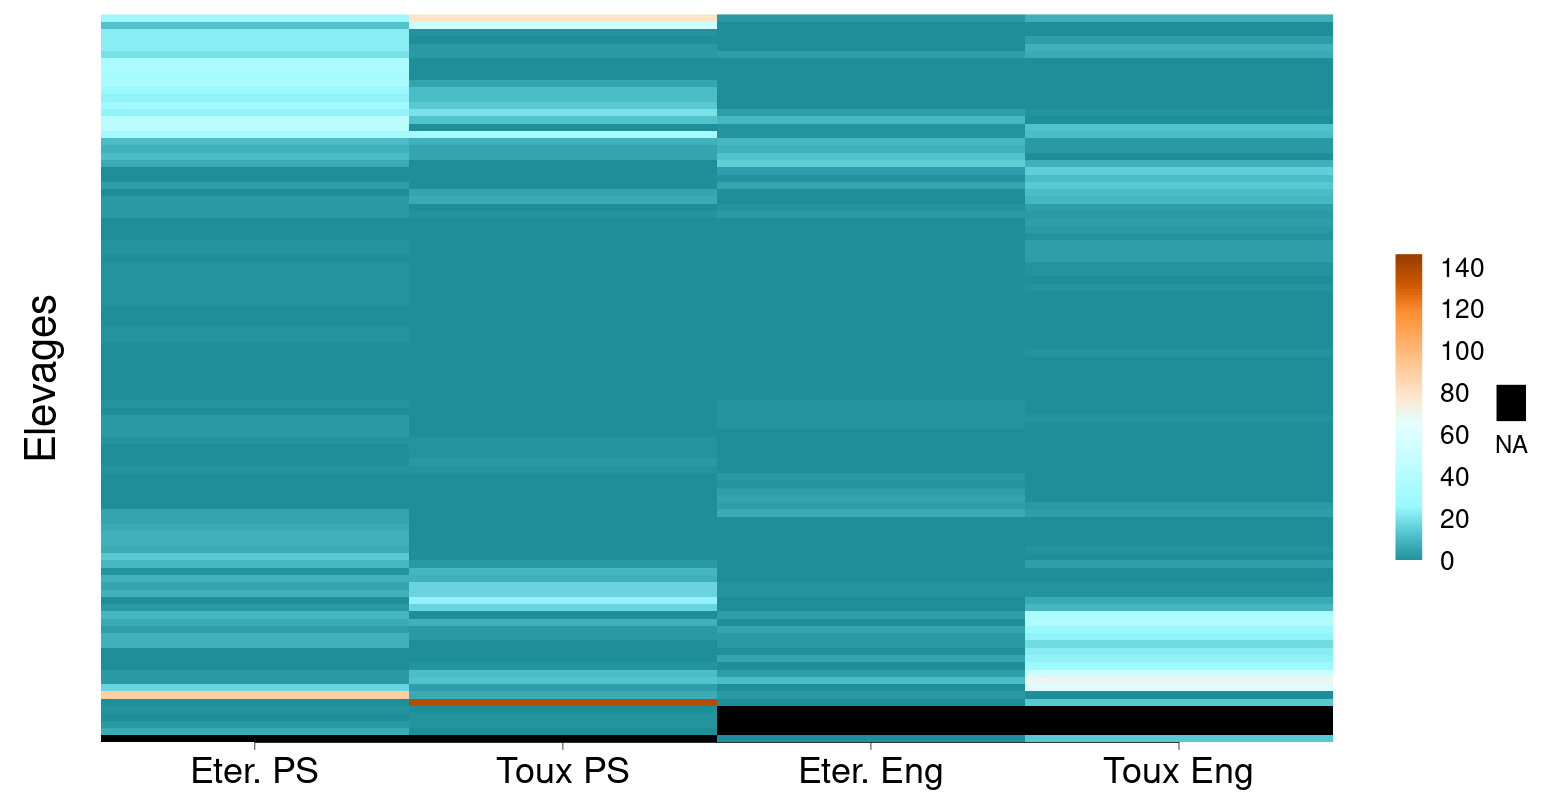
\includegraphics[width=0.9\textwidth]{img_var_resp/rep_var_resp.png}
    \caption{Visualisation des variables respiratoires par élevages}\label{fig:rep_resp}
\end{figure}
Dans (\ref{fig:rep_resp}), nous constatons une fois de plus que la majorité des individus présentent des valeurs faibles pour l'ensemble des variables respiratoires. Nous relevons également la présence de cinq individus avec des valeurs manquantes. Il apparaît que ces valeurs manquantes concernent soit les variables issues de l'engraissement, soit celles du post-sevrage. Cette observation est cohérente avec le protocole de l'étude, qui prévoyait la mesure simultanée des éternuements et des toux.
Des légères corrélations entre la toux et les éternuements sont également observées au sein d'un même lot.
\subsection{Exploration des relations entre les variables respiratoires}
L'objectif de cette section est d'analyser la force des liens entre les variables respiratoires, afin de déterminer si une régression linéaire pourrait être pertinente pour réduire le nombre de variables à considérer dans les étapes suivantes. De plus, cette exploration permet d'évaluer la pertinence de l'Analyse en Composantes Principales (ACP) pour la réduction de dimensions, afin de juger de son adéquation avec nos données.

\subsubsection{Relations linéaires entre les variables respiratoires}
Examinons les corrélations ainsi que la répartition des élevages selon les variables respiratoires.
\begin{figure}[htbp]
    \centering
    \begin{subfigure}[b]{0.49\textwidth}
        \centering
        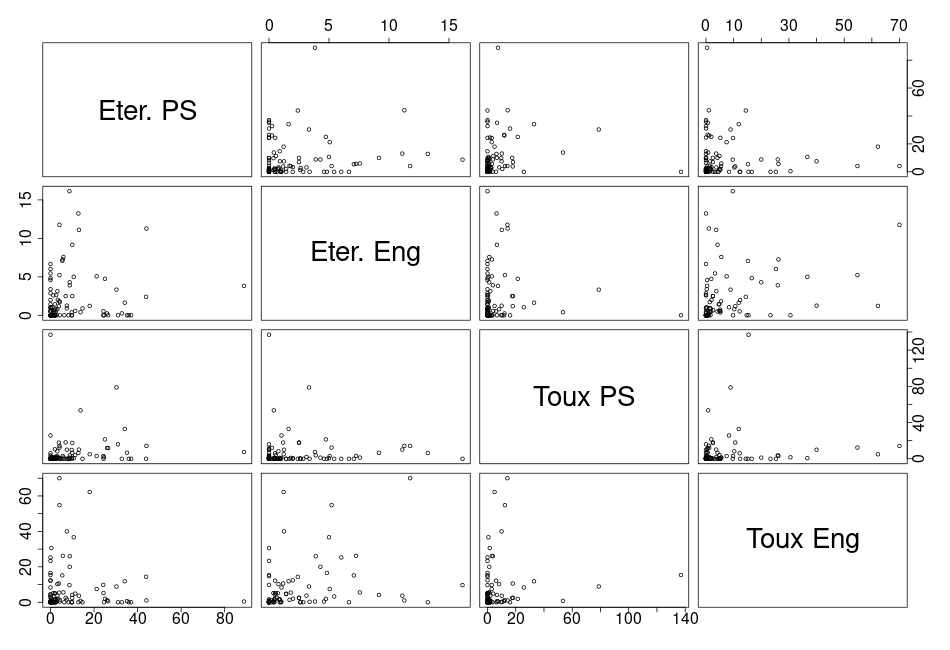
\includegraphics[width=\textwidth]{img_var_resp/points_corr_lin.png}
        \caption{Répartition des élevages}\label{fig:disp_lin}
    \end{subfigure}
    \hspace{0.1cm}
    \begin{subfigure}[b]{0.49\textwidth}
        \centering
        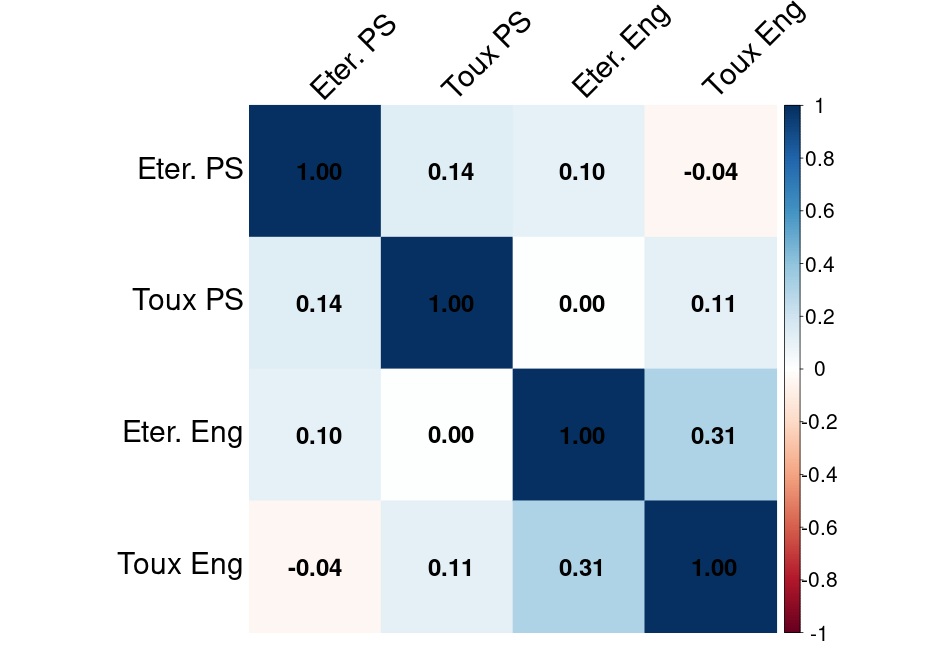
\includegraphics[width=\textwidth]{img_var_resp/corrplot_corr_lin.png}
        \caption{Matrice des correlations}\label{fig:corr_mat_lin}
    \end{subfigure}
    \caption{Illustration étude linéaire}\label{fig:etu_lin}
\end{figure}

Dans la figure (\ref{fig:etu_lin}), aucune relation linéaire forte n’apparaît entre les différentes variables. Ce constat est particulièrement évident dans la figure (\ref{fig:disp_lin}), où les nuages de points ne présentent pas la structure triangulaire typique d’une dispersion linéaire.
Cependant, la matrice de corrélation (\ref{fig:corr_mat_lin}) met en évidence des faibles corrélations entre la plupart des variables, à l’exception notable des éternuements en engraissement et des toux en post-sevrage. On observe en effet une corrélation marquée entre les toux et les éternuements, qui appartiennent au même groupe (soit engraissement, soit post-sevrage), cette corrélation étant particulièrement prononcée chez les porcs en engraissement.
Le test de Pearson confirme ces observations (Cf.\text{ }\ref{annexe:pearson}): la seule corrélation statistiquement significative concerne les variables toux et éternuements en engraissement.

Les analyses graphiques et le test de Pearson révèlent une absence de relations linéaires globales entre les variables, à l'exception de la corrélation entre toux et éternuements en engraissement. Par conséquent, l'ACP, qui repose sur des hypothèses de linéarité, ne semble pas être la méthode d'analyse la mieux adaptée à ce jeu de données.


\subsubsection{Relations logarithmiques entre les variables respiratoires}


\subsection{Analyse des regroupements: réduction de dimensions et catégorisation}

\newpage
\appendix

\section{Annexe: compléments de l'analyse sur les variables respiratoires}
\subsection{Test de pearson sur les corrélations des variables réspiratoires}\label{annexe:pearson}

\begin{table}[ht]
    \centering
    \begin{tabular}{llccc}
    \toprule
    \textbf{Variable 1} & \textbf{Variable 2} & \textbf{Coefficient de corrélation} & \textbf{p-valeur} & \textbf{Significatif} \\
    \midrule
    Eter. PS & Eter. Eng & 0.104 & 0.317 & Non \\
    Eter. PS & Toux PS & 0.135 & 0.191 & Non \\
    Eter. PS & Toux Eng & -0.041 & 0.696 & Non \\
    Eter. Eng & Toux PS & 0.003 & 0.979 & Non \\
    Eter. Eng & Toux Eng & 0.305 & 0.003 & Oui \\
    Toux PS & Toux Eng & 0.114 & 0.273 & Non \\
    \bottomrule
    \end{tabular}
    \caption{Résultats des tests de corrélation de Pearson entre les variables respiratoires.}\label{tab:correlation_results}
\end{table}
Constatons que la seule corrélation significative est celle des variables de toux et éternouments en engraissement. 

\end{document}
